
\subsection{First Come First Served}
\markright{\thesubsection\quad First Come First Served} % Manually update \rightmark
For first, we analyze the First Come First Served (FCFS) scheduling policy. 
In the next section we will analyze the Shortest Job First (SJF) policy and compare
the two scenarios.
\subsubsection{Turnaround time}

The first metric to be analyzed is the turnaround time.
From \cref{fig:fcfsTurnEcdf} and \cref{fig:fcfsTurnDensity} we can see that a larger utilization of the CPUs $\rho$ 
skews the distribution of turnaround time to the right. This can be explained 
by the fact that the more the CPUs are utilized, the more probable is for a
process to be queued and to wait more.
The effects of $\rho$ are more pronounced with fewer CPUs (as expected), and a higher 
\texttt{pCpuBound}. In fact, with a higher \texttt{pCpuBound} a process spends 
most of its time in the CPU, increasing the probability of forming a queue of 
ready processes.

\begin{figure}[H]
    \captionsetup{type=figure}
    \centering
    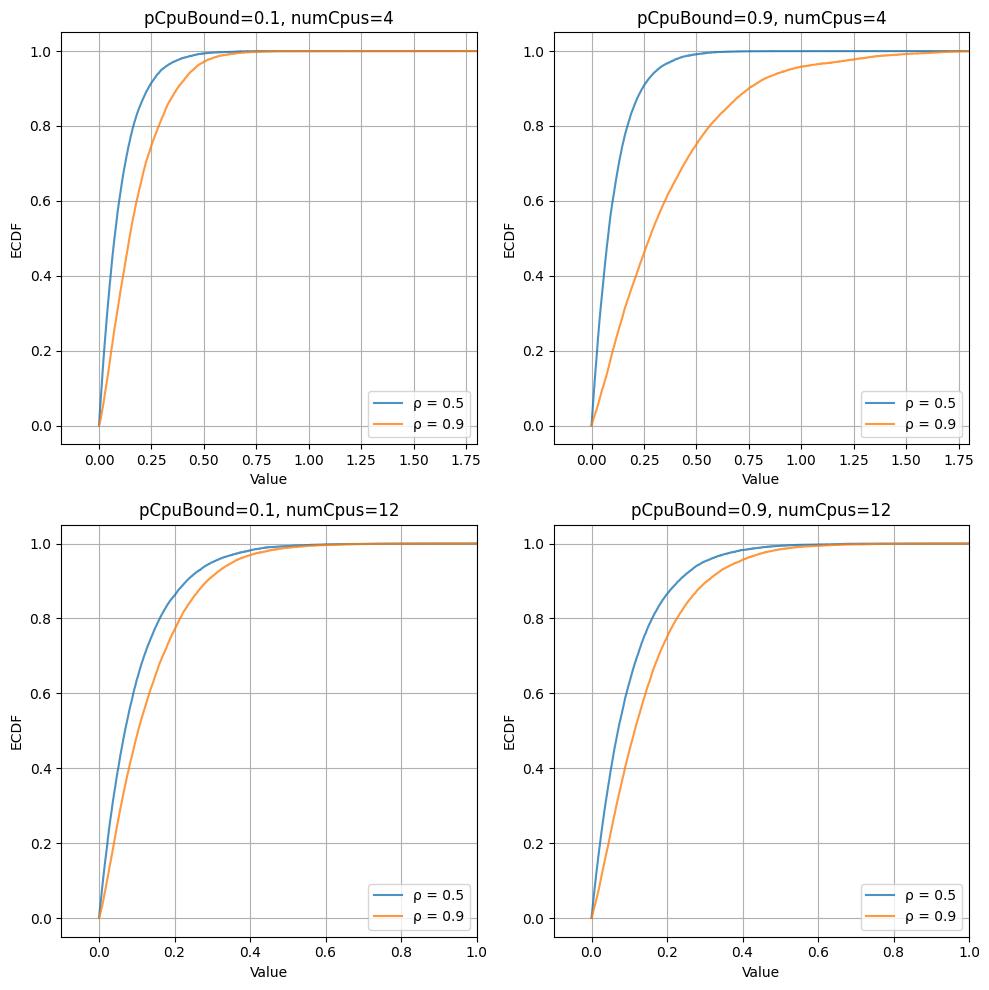
\includegraphics[width=0.9\textwidth]{./images/04/fcfs/turn/ecdf.png}
    \caption{Empirical CDF of the turnaround time of the systems.}
    \label{fig:fcfsTurnEcdf}
\end{figure}

The empirical probability density function of the turnaround time, shown
in \cref{fig:fcfsTurnDensity}, confirms the previous observations. Comparing
the plot above to the right with the others, we can observe that
the distribution is more uniform and skewed to the right when $\rho$ is higher,
the processes are more likely CPU bound and there are few CPUs. In this case, 
the turnaround time can be modeled as the sum of the waiting time in the queue with the 
service time of the process. 

When, instead, the utilization and the \texttt{pCpuBound} are lower and the 
number of CPUs is higher, the distribution is approximately an exponential:
in this case the effects of queueing are less pronounced and the turnaround time
is mainly determined by the (exponential) service time of the process.

\begin{figure}[H]
    \captionsetup{type=figure}
    \centering
    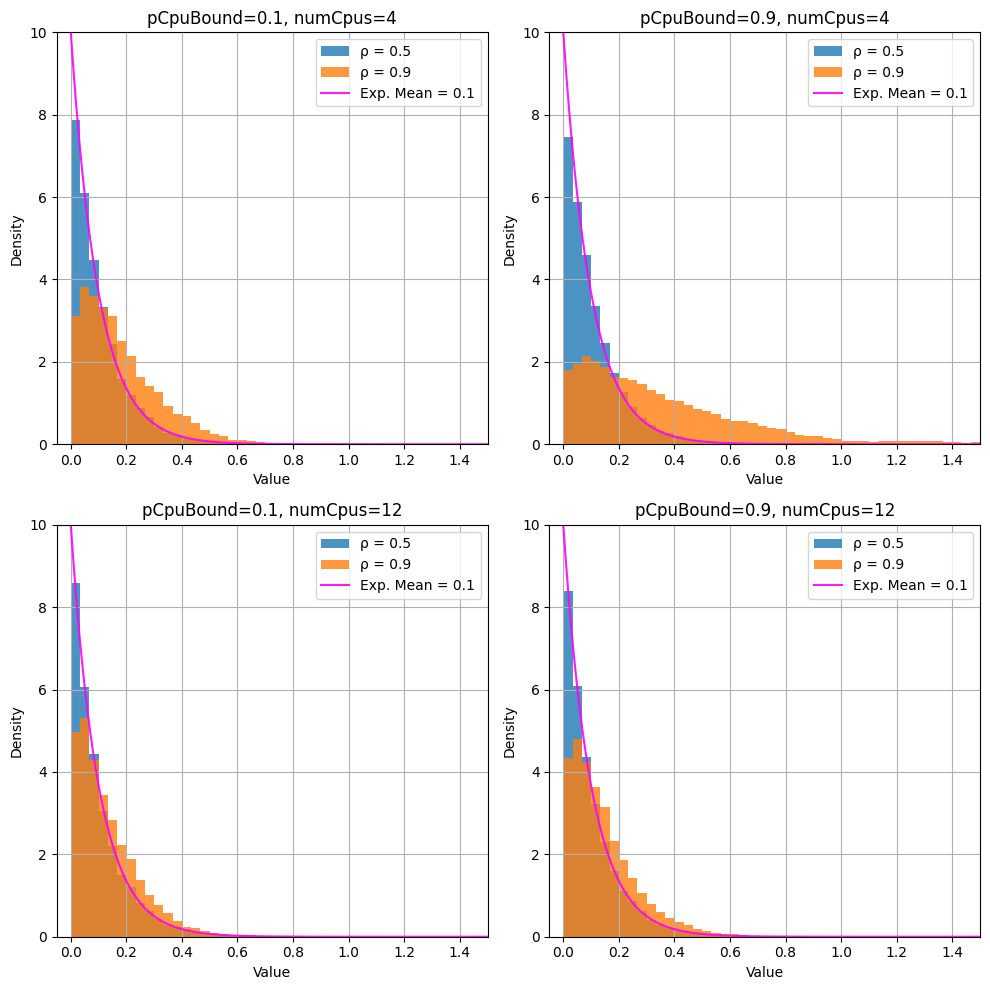
\includegraphics[width=0.9\textwidth]{./images/04/fcfs/turn/density.png}
    \caption{Density plot of the turnaround time of the systems.}
    \label{fig:fcfsTurnDensity}
\end{figure}

From the Lorenz curve in \cref{fig:fcfsTurnLorenz} we can see that the 
distribution that the turnaround time assumes with bigger $\rho$ is more fair 
than the one with smaller $\rho$. We can explain this by the fact that when the
system is more utilized, the processes are more likely to be queued and to wait
a similar amount of time, making the distribution more fair.

\begin{figure}[H]
    \captionsetup{type=figure}
    \centering
    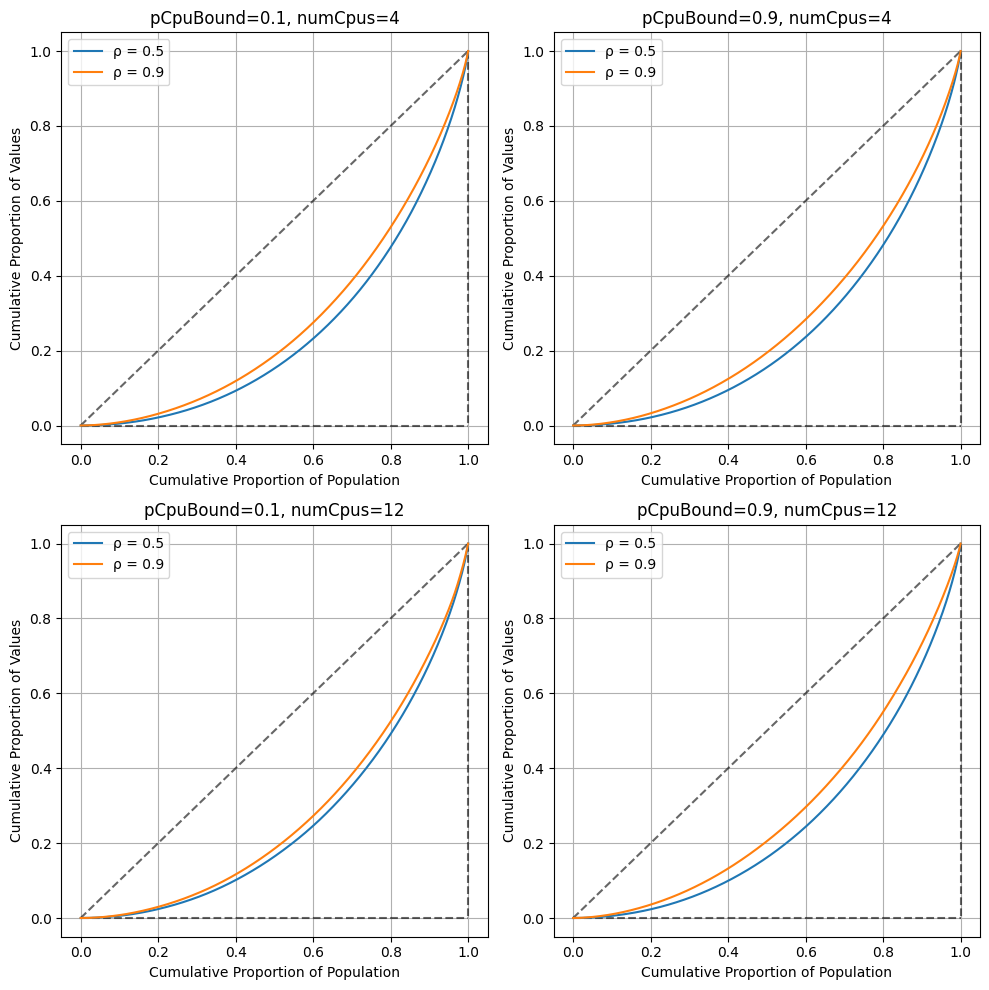
\includegraphics[width=0.7\textwidth]{./images/04/fcfs/turn/lorenz.png}
    \caption{Lorenz curve of the turnaround time of the systems.}
    \label{fig:fcfsTurnLorenz}
\end{figure}

In \cref{fig:fcfsTurnAutocorrelation} we see 
that larger $\rho$ values make the distribution more correlated, while more 
CPUs and a lower \texttt{pCpuBound} make the distribution less correlated.

This fits perfectly with the model: when the system is more utilized, the
processes are more likely to be queued, so the waiting time of
each process will be closely related to the one of its nearest 
processes in the queue, making the distribution
more correlated. When the system is less utilized, the processes are more likely
to be served immediately, making the distribution dependent only on the service
time of the process.

\begin{figure}[H]
    \captionsetup{type=figure}
    \centering
    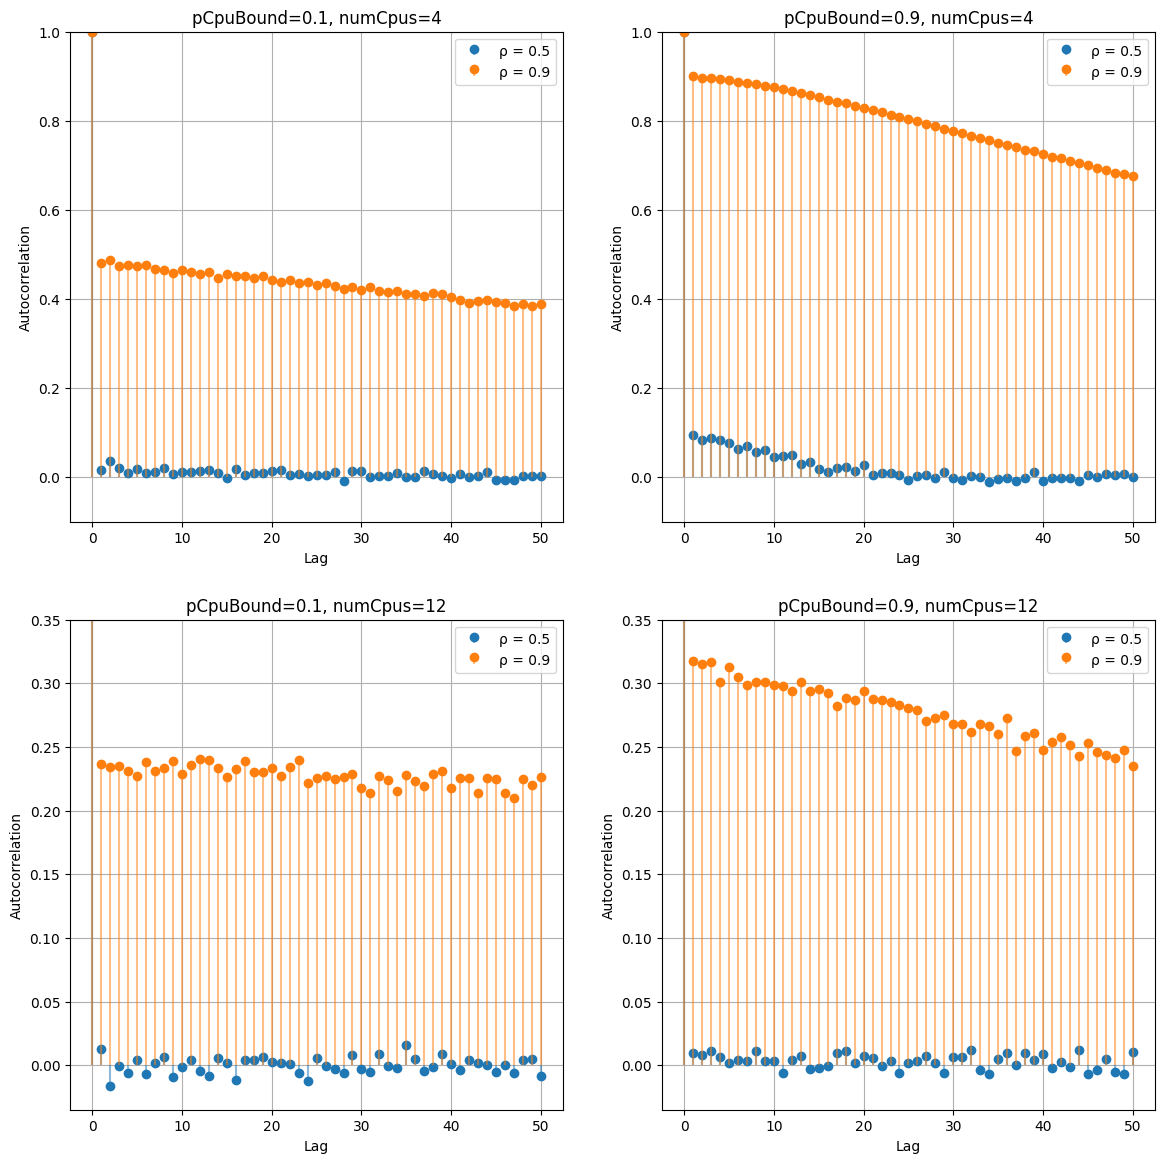
\includegraphics[width=0.7\textwidth]{./images/04/fcfs/turn/autocorrelation.png}
    \caption{Autocorrelation plot of the turnaround time of the systems.}
    \label{fig:fcfsTurnAutocorrelation}
\end{figure}

After using subsampling to make the data uncorrelated, we used bootstrap to calculate the confidence intervals of the mean and the standard deviation of the turnaround time. The \texttt{std dev} was calculated since we expect it to be equal to the mean when the distribution is exponential. It can be seen in \cref{tab:fcfsTurn} that for small $\rho$ they are similar.

\begin{table}[H]
    \centering
    \scriptsize
    \begin{tabular}{llc|c|c|c|c|c|c|c}
\toprule
& & \multicolumn{4}{c|}{numCpus = 4} & \multicolumn{4}{c}{numCpus = 12} \\
& & \multicolumn{2}{c|}{pCpuBound = 0.1} & \multicolumn{2}{c|}{pCpuBound = 0.9} & \multicolumn{2}{c|}{pCpuBound = 0.1} & \multicolumn{2}{c}{pCpuBound = 0.9} \\
Index & & $\rho = 0.5$ & $\rho = 0.9$ & $\rho = 0.5$ & $\rho = 0.9$ & $\rho = 0.5$ & $\rho = 0.9$ & $\rho = 0.5$ & $\rho = 0.9$ \\
\midrule
\multirow{3}{*}{Mean} & Value & 103.1 & 195.0 & 108.5 & 358.4 & 99.6 & 132.5 & 100.1 & 144.6 \\
& 95\% CI Low & 101.2 & 181.2 & 102.3 & 321.2 & 97.7 & 121.5 & 98.6 & 131.4 \\
& 95\% CI High & 105.3 & 211.5 & 114.5 & 395.7 & 101.6 & 146.0 & 101.4 & 158.2 \\
\midrule
\multirow{3}{*}{Std Dev} & Value & 101.3 & 137.2 & 108.1 & 316.6 & 99.3 & 113.5 & 98.8 & 126.7 \\
& 95\% CI Low & 98.6 & 126.2 & 102.2 & 280.2 & 96.7 & 102.4 & 97.0 & 111.8 \\
& 95\% CI High & 104.1 & 152.1 & 115.1 & 365.0 & 102.0 & 127.6 & 100.6 & 145.3 \\
\bottomrule
\end{tabular}
    \caption{Bootstrap results for turnaround time mean and Std Dev. (ms)}
    \label{tab:fcfsTurn}
\end{table}


\subsubsection{Waiting time}

From \cref{fig:fcfsWaitEcdf} and \cref{fig:fcfsWaitDensity} it is clear to see that 
for $\rho = 0.5$ the waiting time is almost always $0$. For this reason in 
\cref{fig:fcfsWaitLorenz} we see that the waiting time is more unfair when $\rho$ 
is lower, since this is the behaviour of the line of maximum unfairness 
(all values equal to 0 except for one). In \cref{fig:fcfsWaitAutocorrelation} we 
see that even when $\rho = 0.5$ the times are really correlated.

\begin{figure}[H]
    \captionsetup{type=figure}
    \centering
    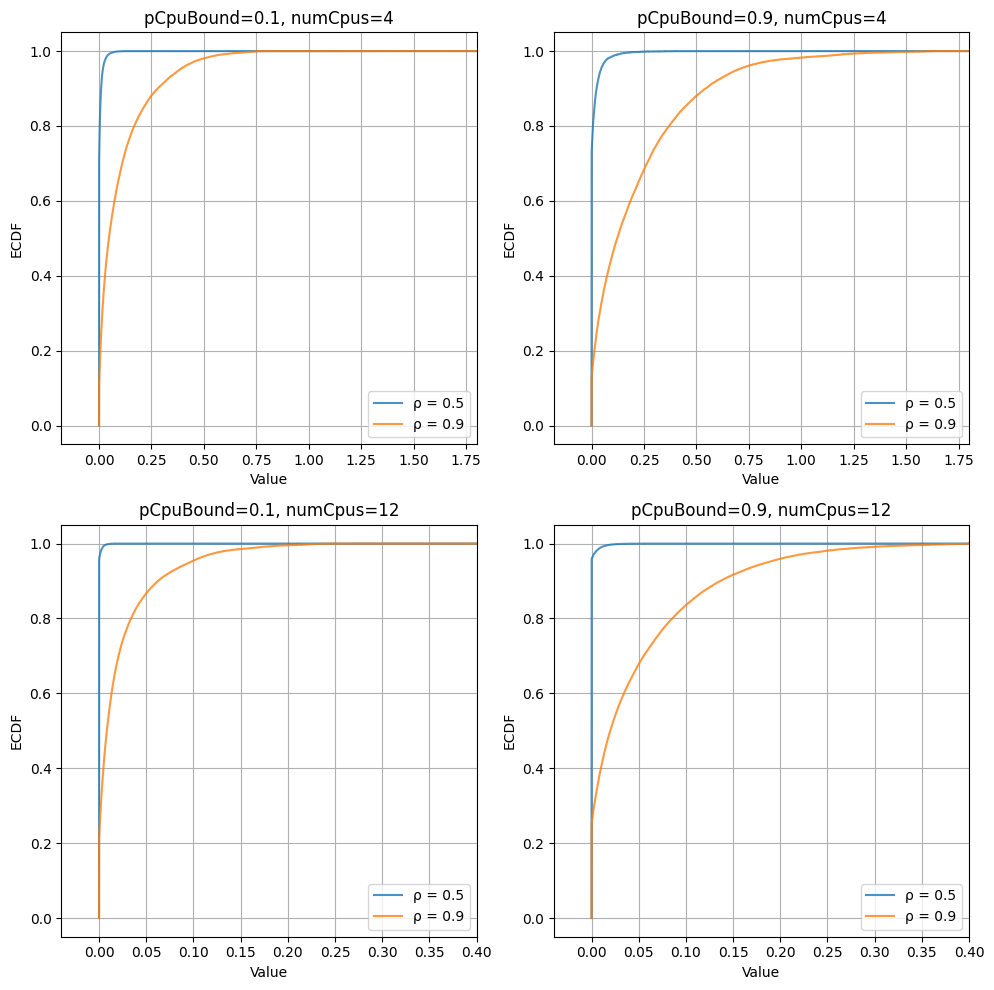
\includegraphics[width=0.85\textwidth]{./images/04/fcfs/wait/ecdf.png}
    \caption{Empirical CDF of the waiting time of the systems.}
    \label{fig:fcfsWaitEcdf}
\end{figure}

From the plots of the empirical CDF it is possible to observe that the utilization
of the CPUs impacts more than the variation of the single parameters \texttt{pCpuBound}
and \texttt{numCpus} on the waiting time. Anyway, looking from left to
right in particular at the impact of the first parameter, the time of CPU processing increases
and the distribution moves to the higher values.

\begin{figure}[H]
    \captionsetup{type=figure}
    \centering
    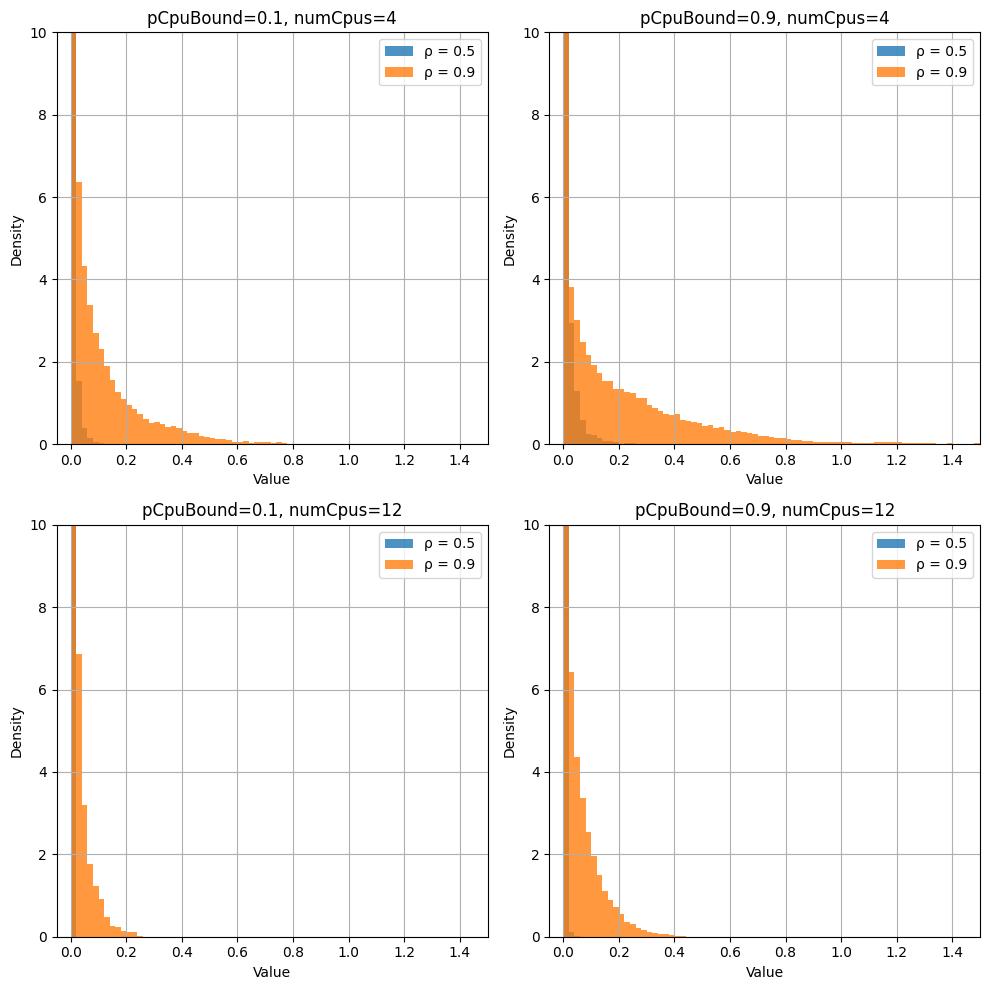
\includegraphics[width=0.7\textwidth]{./images/04/fcfs/wait/density.png}
    \caption{Density plot of the waiting time of the systems.}
    \label{fig:fcfsWaitDensity}
\end{figure}

The analysis of the probability density function of the waiting time confirms
that at low values of $\rho$ the process are almost never queued. From left below to
right above, the distribution is more uniform and skewed to the right, with the density
concentrated less around the value 0.


\begin{figure}[H]
    \captionsetup{type=figure}
    \centering
    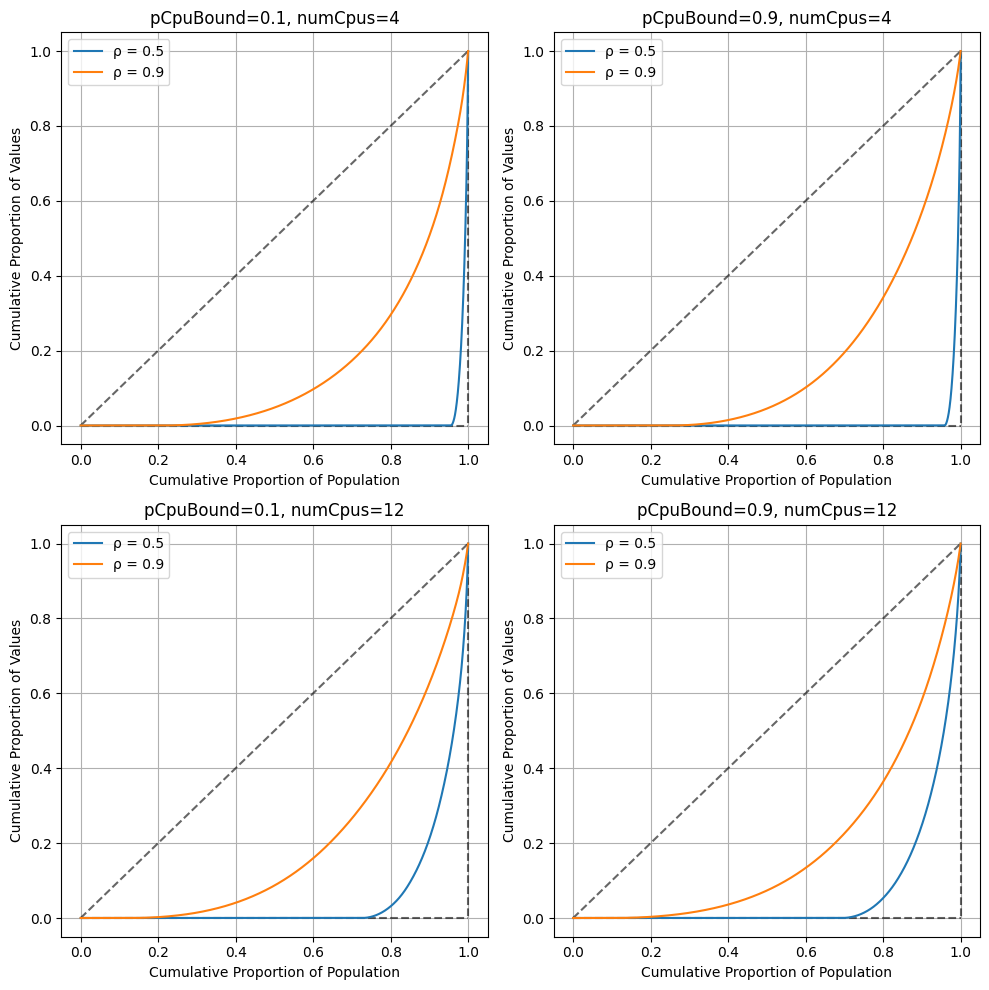
\includegraphics[width=0.9\textwidth]{./images/04/fcfs/wait/lorenz.png}
    \caption{Lorenz curve of the waiting time of the systems.}
    \label{fig:fcfsWaitLorenz}
\end{figure}

We also analyzed the unfairness of the distribution of the wating time in the 
different scenarios, plotting the Lorenz curves in \cref{fig:fcfsWaitLorenz}.
In every case the distribution is more unfair when $\rho$ is lower, since the
waiting time is almost always $0$. 

\begin{figure}[H]
    \captionsetup{type=figure}
    \centering
    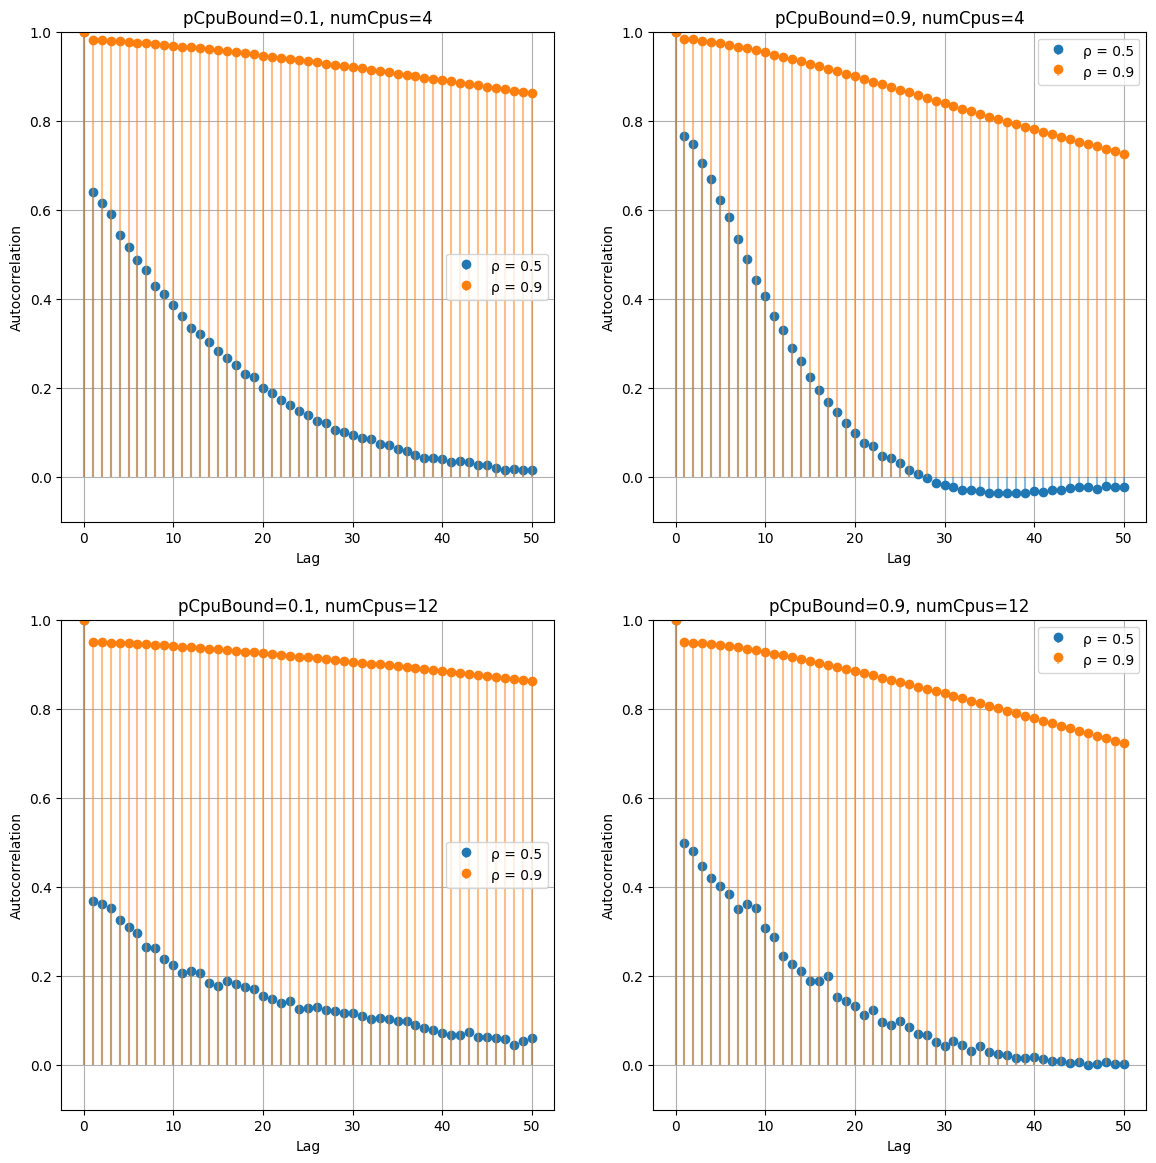
\includegraphics[width=0.7\textwidth]{./images/04/fcfs/wait/autocorrelation.png}
    \caption{Autocorrelation plot of the waiting time of the systems.}
    \label{fig:fcfsWaitAutocorrelation}
\end{figure}

The observation of the autocorrelation of the waiting time has been done with the 
lag plots in \cref{fig:fcfsWaitAutocorrelation}. With high utilization,
the correlation is always high and this reflects the expectations: if a process has
waited a long time, the next one will probably wait a long time too. When the system
is less utilized, the correlation is lower, since queuing is less likely.

\begin{table}[H]
    \centering
    \scriptsize
    \begin{tabular}{llc|c|c|c|c|c|c|c}
\toprule
& & \multicolumn{4}{c|}{numCpus = 4} & \multicolumn{4}{c}{numCpus = 12} \\
& & \multicolumn{2}{c|}{pCpuBound = 0.1} & \multicolumn{2}{c|}{pCpuBound = 0.9} & \multicolumn{2}{c|}{pCpuBound = 0.1} & \multicolumn{2}{c}{pCpuBound = 0.9} \\
Index & & $\rho = 0.5$ & $\rho = 0.9$ & $\rho = 0.5$ & $\rho = 0.9$ & $\rho = 0.5$ & $\rho = 0.9$ & $\rho = 0.5$ & $\rho = 0.9$ \\
\midrule
\multirow{3}{*}{Mean} & Value & 2.7 & 92.4 & 5.8 & 213.0 & 0.1 & 21.2 & 0.3 & 43.0 \\
 & 95\% CI Low & 2.3 & 81.6 & 4.7 & 186.1 & 0.1 & 18.0 & 0.2 & 36.9 \\
 & 95\% CI High & 3.3 & 103.7 & 8.1 & 242.7 & 0.2 & 25.0 & 0.6 & 50.4 \\
\midrule
\multirow{3}{*}{Std Dev} & Value & 7.8 & 108.9 & 21.5 & 252.7 & 0.9 & 35.4 & 2.2 & 64.8 \\
 & 95\% CI Low & 6.4 & 99.4 & 14.4 & 221.6 & 0.6 & 30.8 & 1.3 & 56.6 \\
 & 95\% CI High & 9.4 & 120.4 & 36.2 & 300.0 & 1.3 & 43.0 & 4.2 & 75.3 \\
\bottomrule
\end{tabular}

    \caption{Bootstrap results for waiting time mean and Std Dev. (ms)}
    \label{tab:fcfsWait}
\end{table}

The quantitative analysis of the waiting time in the exponential case is reported in 
\cref{tab:fcfsWait}. Of course, with same duration of the processes and same
utilization, the more each process spends in the CPU, the more the processes
meanly waits in the queue. So with high \texttt{pCpuBound} and low \texttt{numCpus}
the mean value of the waiting time increases.

Since the confidence intervals of the mean value and of the standard deviation do 
not overlap, we can infer that the distribution is not exponential.

\subsubsection{CPU utilization}

\label{sec:fcfsCpuUtilization}

\begin{table}[H]
    \centering
    \scriptsize
    \begin{tabular}{lc|c|c|c|c|c|c|c}
\toprule
& \multicolumn{4}{c|}{numCpus = 4} & \multicolumn{4}{c}{numCpus = 12} \\
& \multicolumn{2}{c|}{pCpuBound = 0.1} & \multicolumn{2}{c|}{pCpuBound = 0.9} & \multicolumn{2}{c|}{pCpuBound = 0.1} & \multicolumn{2}{c}{pCpuBound = 0.9} \\
Index & $\rho = 0.5$ & $\rho = 0.9$ & $\rho = 0.5$ & $\rho = 0.9$ & $\rho = 0.5$ & $\rho = 0.9$ & $\rho = 0.5$ & $\rho = 0.9$ \\
\midrule
Mean & 2.02 & 3.61 & 2.03 & 3.63 & 6.01 & 10.82 & 6.03 & 10.80 \\
\midrule
Std Dev & 1.30 & 0.88 & 1.30 & 0.86 & 2.43 & 1.99 & 2.45 & 2.00 \\
\bottomrule
\end{tabular}
    \caption{Mean and Std Dev of number of busy cpus.}
    \label{tab:fcfsCpus}
\end{table}

We see that the obtained values are inline with the theoretical model:
\begin{equation}
    \rho * numCpus = meanCpuUtilized
\end{equation}


For example, in the second column, $0.9 * 4 \approx 3.61$ 

\subsubsection{Ready queue length}

In \cref{tab:fcfsReadyProc} it is reported the mean and the standard deviation 
of the number of ready processes in the queue. 

\begin{table}[H]
    \centering
    \scriptsize
    \begin{tabular}{lc|c|c|c|c|c|c|c}
\toprule
& \multicolumn{4}{c|}{numCpus = 4} & \multicolumn{4}{c}{numCpus = 12} \\
& \multicolumn{2}{c|}{pCpuBound = 0.1} & \multicolumn{2}{c|}{pCpuBound = 0.9} & \multicolumn{2}{c|}{pCpuBound = 0.1} & \multicolumn{2}{c}{pCpuBound = 0.9} \\
Index & $\rho = 0.5$ & $\rho = 0.9$ & $\rho = 0.5$ & $\rho = 0.9$ & $\rho = 0.5$ & $\rho = 0.9$ & $\rho = 0.5$ & $\rho = 0.9$ \\
\midrule
Mean & 0.25 & 13.72 & 0.22 & 10.27 & 0.03 & 9.81 & 0.03 & 7.19 \\
\midrule
Std Dev & 0.96 & 18.47 & 0.89 & 12.99 & 0.29 & 16.34 & 0.28 & 10.57 \\
\bottomrule
\end{tabular}

    \caption{Mean and Std Dev of number of ready processes in queue.}
    \label{tab:fcfsReadyProc}
\end{table}

The values are in line with the theoretical model. In fact, applying Little's Law and computing the ratio between
$E[N_q]$ and the arrival rate, the values obtained are coherent with the mean of
the waiting time described in \cref{tab:fcfsWait}.